\newcommand{\name}{K221 -- Mö\ss bauer Effect}
\documentclass[11pt,a4paper,notitlepage]{scrartcl}
\usepackage{DasPaket}
\title{ Advanced Laboratory Course}
\subtitle{\name  \\ \hrulefill}
\date{May 19. 2021\\}
%\date{Date of Experiment \\ \sectionlinetwo{black}{88}}
\author[*]{\textsc{Dominic Schüchter}}
\author[$\dagger$]{\textsc{Jakob Krause}}
\affil[*]{\href{mailto:dschuechter@uni-bonn.de}{\faEnvelope  \hspace*{0.1cm}dschuechter@uni-bonn.de} {\color{black}$|$} \href{https://github.com/dschuechter}{\faGithub  \hspace*{0.1cm}dschuechter}}
\affil[$\dagger$]{\href{mailto:krause.jakob@uni-bonn.de}{\faEnvelope  \hspace*{0.1cm}krause.jakob@uni-bonn.de} {\color{black}$|$} \href{https://github.com/krausejm}{\faGithub  \hspace*{0.1cm}krausejm}}
\usepackage{blindtext}
\graphicspath{{figs/}}
\usepackage{mathtools}
\addbibresource{Literatur.bib}
\usepackage{longtable}
\begin{document}

\maketitle
\vspace{-.8cm}
\thispagestyle{empty}
\begin{center}
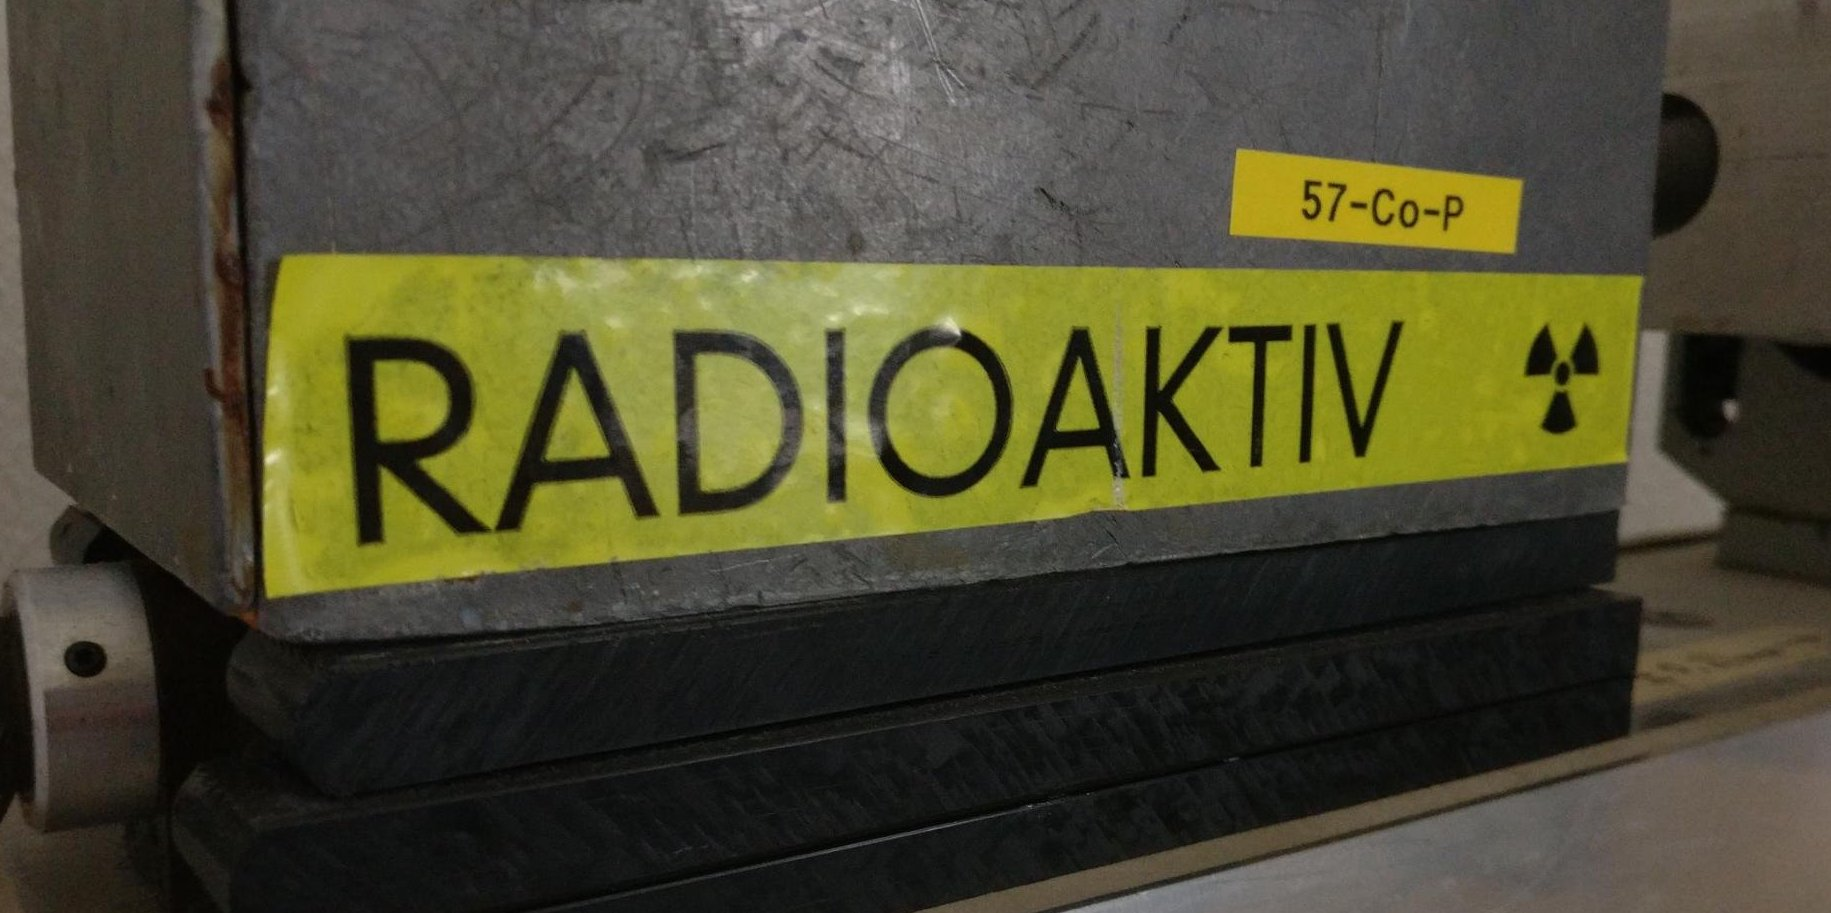
\includegraphics[width=\linewidth]{God}
\vspace{-.2cm}

\rule{12cm}{1pt} \\\vspace{-.6cm} \rule{10cm}{1pt}
\end{center}



\begin{abstract}
	In this report we investigated the \textsc{Mö\ss bauer} effect -- a recoilless emission/absorption of photons by nuclei. We used the $^{57}$Co isotope that decays into the excited  $^{57}$Fe  and investigated it's 14.4keV line as a result of the transition between the first excited to ground state. Further we used the taken \textsc{Mö\ss bauer} spectrum to derive properties of electric and magnetic single and multipole properties like the $g$-factor and the natural linewidth $\Gamma$.
\end{abstract}
\begin{center}
	 \rule{10cm}{1pt} \\\vspace{-.6cm} \rule{12cm}{1pt}
\end{center}

\setcounter{page}{-1}
\newpage

\tableofcontents
\thispagestyle{empty}
\newpage
\section{Introduction}
In this experiment we investigated the recoilless $\gamma$ emission and absorption of nuclei, the so called \textsc{Mö\ss bauer}-effect. With the used techniques of this experiment we were able to measure the natural linewidth of the $^{57}$Fe transition to ground state at 14.4keV and investigate electric and magnetic single and multipole influences. Additionally we derived the \textsc{Lande}-factor $g$ for the hyperfine structure of the ground and first excited state of this isotope.

This lab report will introduce you into the fundamental theories behind the \textsc{Mö\ss bauer}-effect and -spectroscopy. The used experimental setup will be explained and the taken data presented and analyzed. Finally we briefly summarize the results and compare them to the literature values.
\newpage

\section{Theory}\label{sec:theory}
In this section we will give a brief introduction into the theory behind this experiment. This only gives the most important informations and equations needed for the later analysis. Knowledge of the \textsc{Doppler}-effect is required. For more detailed informations look e.g. \cite{chemistry} or \cite{schatz}.
\subsection{Mö\ss bauer effect}
The \textsc{Mö\ss bauer}-effect is --as introduced-- the recoilless emission/absorption of photons by nuclei. The fundamentals of physics are based on energy and momentum conservation. If a free, resting and excited nucleus transitions into its ground state via emitting a photon, its momentum changes in the opposite direction to the emitted photon. The energy of the photon is therefore smaller then the energy difference between the excited and ground state. If this photon encounters another free, resting nucleus at ground state of the same kind, the energy would now be to small to excite it. The same goes for a photon with a matching energy and a free, resting nucleus in ground state. Again --because of momentum conservation-- would the energy of the photon converted into kinetic energy of the nucleus. For free, resting nuclei would therefore a resonant transition not be possible.

The \textsc{Mö\ss bauer}-effect gives a smart workaround for this problem. If the nuclei are part of a crystalline structure, the recoil energies are transferred into the whole crystal. The recoil becomes negligible for the high crystal mass. Resonant transitions are possible. \cite{chemistry}
\subsection{Debye-Waller-factor}\label{sec:debye}
The \textsc{Debye-Waller}-factor $f$ is defined as the ratio between the recoilless emitted/absorbed $\gamma$'s to all and is therefore the probability of the \textsc{Mösbauer}-effect \cite{chemistry}. For low temperatures ($T<\Theta$) the \textsc{Debye-Waller}-factor can be written as \cite{schatz}:
\begin{equation*}
	f(T)=\exp\left\{-\frac{\hbar^2\cdot k^2}{2M}\frac{3}{2k_B\Theta}\left[1+\frac{2\pi^2}{3}\left(\frac{T}{\Theta}\right)^2\right]\right\}
\end{equation*}
\begin{center}
		with the \textsc{Debye}-temperature $\Theta$, temperature $T$, the atom mass $M$, \textsc{Boltzmann}. constant $k_B$
\end{center}

In general is this factor anti proportional to the temperature $T$ and the photon energy $E_\gamma$ ($\hbar\cdot k=\frac{E_\gamma}{c}$). The \textsc{Debye-Waller}-factor is an important property of the used material. \cite{schatz}

With the \textsc{Debye}-temperature for Iron $\Theta_{\text{Fe}}=470K$ \cite{solids} and the energy $E_\gamma=14.4keV$ follows:
$$f(T)\approx 0.78$$
This value is a good sign for the material choice, since we get at room temperatures sufficient values. One could improve this result by cooling done the source and absorber.
\newpage
\subsection{The Mö\ss bauer-source -- $^{57}$Co-Decay scheme}
\begin{wrapfigure}[12]{R}{0.5\linewidth}
	\centering
	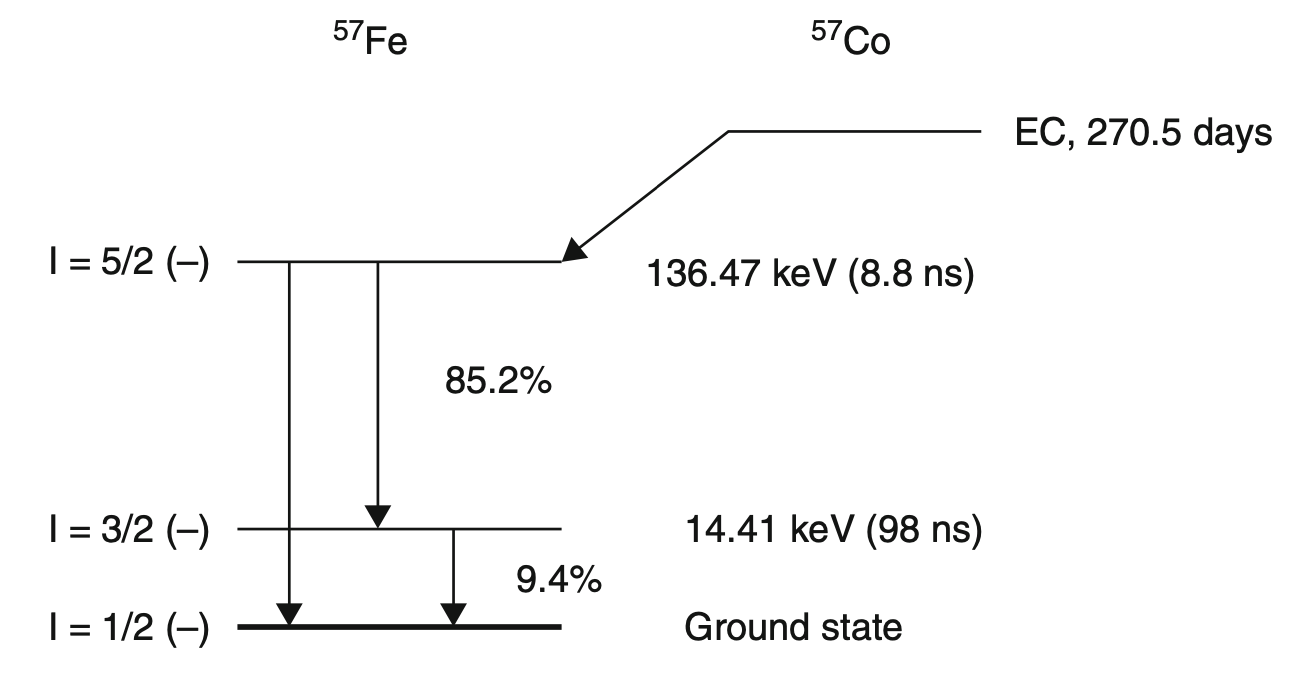
\includegraphics[width=\linewidth]{figs/scheme.png}
	\caption{$^{57}$Co $\to ^{57}$Fe decay scheme \cite{chemistry}}\label{fig:decay_scheme}
\end{wrapfigure}

A proper source to measure the \textsc{Mö\ss bauer}-spectrum requires the following properties \cite{schatz}:
\begin{enumerate}
	\item The observed $\gamma$-transition must lead to the ground state.
	\item The Debye-Waller-factor should not be small
	\item Practical lifetimes of the \textsc{Mö\ss bauer}-level because of resulting high linewidths $\Gamma=\frac{\hbar}{\tau}$
	\item Practical properties of the parent isotope like the lifetime (continuous measurement)
\end{enumerate}
All those properties are fulfilled for the parent isotope $^{57}$Co and the decay product (electron capture) $^{57}$Fe. The decay scheme is show in figure \ref{fig:decay_scheme}. The resulting \emph{coarse} $\gamma$-spectrum will contain three peaks. The resulting electron cascade will lead to a photopeak at $\approx 6$keV, the peak of interest at $14.4$keV and the simultanious measurement of both events. The transition from $|I=5/2\rangle\to|I=3/2\rangle$ or $|I=5/2\rangle\to|I=1/2\rangle$ result in energies that are not of interest and experimental configuration.

The transition of interest is the \textsc{Mö\ss bauer}-level $|I=3/2\rangle$ to ground state $|I=1/2\rangle$ which results in a photon with energy of 14.4keV. The transition time is long enough to build a sharp line profile. \cite{schatz}
\subsection{The Mö\ss bauer-spectrum and its influences}\label{sec:spectrum}

The \textsc{Mö\ss bauer} spectrum isn't just a single line at 14.4keV. There are multiple effects due to electric and magnetic mono- and multipole effects happening \cite{chemistry}:
\begin{itemize}
	\item \textbf{magnetic dipole interaction}
	Because our probe nuclei are embedded in iron, the ferromagnetic properties of iron apply. The internal magnetic field results in a hyperfine splitting. This results in two hyperfine levels for the ground state with the properties $|I=1/2,m_I=\mp1/2\rangle$ and in four levels for the \textsc{Mö\ss bauer}-state $|I=3/2,m_I=\{\pm1/2,\pm3/2\}\rangle$. With the selection rule $\Delta m_I=0,\pm 1$ \cite{demroeder4} results a hyperfine spectrum of 6 discrete lines.
	The splitting of the energy can be calculated by the equation 
	\begin{equation}\label{eq:hyperfine}
		\Delta E_I=-g_I\cdot B\cdot \mu_N\cdot \Delta m_I
	\end{equation}
	Figure \ref{fig:hyperfine} depicts the hyperfine scheme and the expected spectrum.
	\item \textbf{electric monopole interaction} Because of the nucleus size difference between the excited and ground state, an energy shift occurs due to coulomb interaction primary with lower level electrons. This shift is also called isomeric shift and leads to an asymmetry of the the \textsc{Mö\ss bauer}-spectrum as shown in figure \ref{fig:hyperfine} and described by \cite{chemistry}
	\begin{equation}
		\Delta E_{\text{iso.}}=E_\gamma^{A*}-E_\gamma^{A}
	\end{equation}
	The shift can therefore be easily (as we will later see) derived. \cite{chemistry}
	\item \textbf{electric quadrupole interaction} Because of nonzero nuclear quadrupole moments, our used isotopes are subject to electric quadrupole interaction which are characterized by the electric field gradient. This interaction also results in an energy shift of our spectrum. The resulting shift can be described by the equation
	\begin{equation}\label{eq:quadrupole}
		\Delta E_Q\propto 3m_I^2-I(I+1)
	\end{equation}
	For the ground state with $I=1/2$ and $m_I=\mp1/2$ results a quadrupole shift of $\Delta E_Q=0$. \cite{chemistry}
\end{itemize}
	\begin{figure}[H]
	\centering
	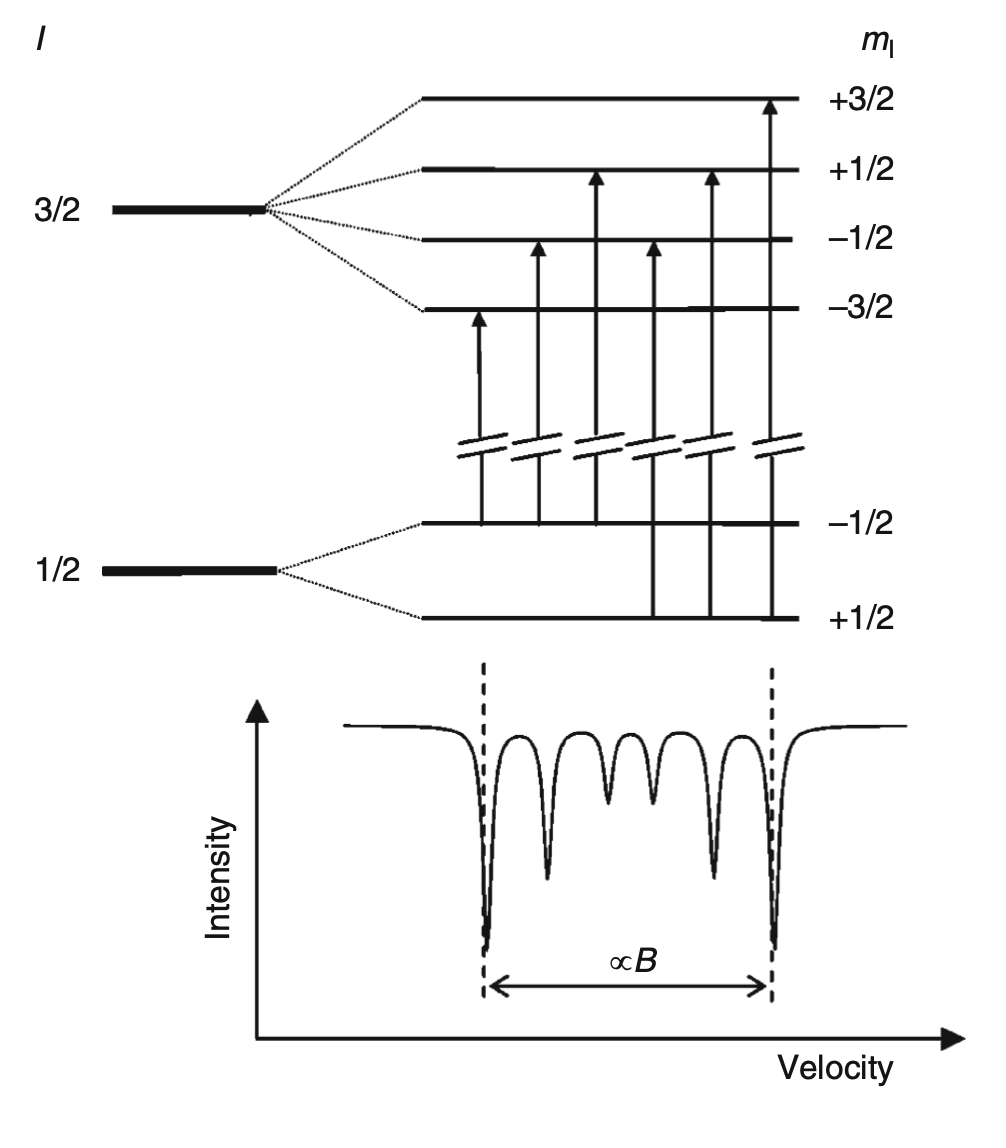
\includegraphics[width=0.5\linewidth]{figs/hyperfine.png}
	\caption{Magnetic dipole interaction/Hyperfine structure of the ground and first excited state of $^{57}$Fe \cite{chemistry}}\label{fig:hyperfine}
\end{figure}
Since our spectrum is the result of resonant absorption/transition the linewidth doesn't get affected by the \textsc{Doppler} broadening and the natural linewidth remains. The natural linewidth is of order $10^{-8}$eV, while a broadened line is about $10^{-2}$eV. Such small linewidth are really hard or impossible to capture with normal detectors without additional work. We will use a smart and surprisingly small setup to do so. \cite{chemistry}
\newpage
\section{Experimental Setup}
\begin{wrapfigure}{R}{0.5\textwidth}
	\centering
	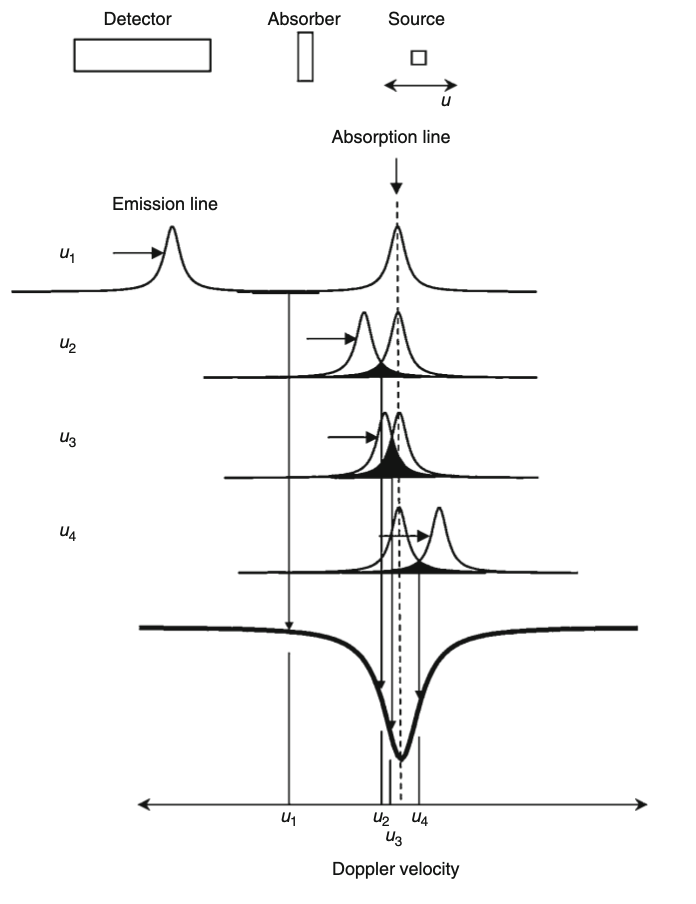
\includegraphics[width=\linewidth]{figs/source.png}
	\caption{Main idea of \textsc{Mö\ss bauer}-spectroscopy \cite{chemistry}}\label{fig:source}
\end{wrapfigure}  
The main idea to measure such small linewidths with high accuracy is to use the \textsc{Doppler} effect. An absorber and a source have resonant transitions. One can scan the peak profile by moving either the source or the absorber to or from the other. By doing so, the wavelength shifts and therefore the frequency of the emitted/received photon. The overlap of the absorber and emitter profiles are directly settling down in the counting rate. Since we measure after the absorber and take an absorption spectrum, the result shall be, that a higher overlap results in a lower counting rate. Figure \ref{fig:source} illustrates this idea. Since the movement is bidirectional and the spectrum is (besides single/multipole influences) symmetric, we can scan through the whole velocity spectrum. \cite{chemistry}

We used in our case a moving absorber with a $^{57}$Fe target and a $^{57}$Co source that is embedded in a metallic matrix. The source was covered by a box with an opening in direction of the absorber and detector. A gasdetector was used to measure the counting rate of $\gamma$'s that is proportional to the voltage amplitude. The motor is controlled by a motorsteering which had a potentiometer to control it's velocity and got gate signals from further electronics (Part 2). Because of the bidirectional configuration, one needs two separate counters. The first one for the movements direction from left to right (LR) and the second one for the movement from right to left (RL). The setup could not guaranty the same speed in LR and RL directions, even with the same steering settings. Therefore was for every run also the time besides the number of counts measured, from which the counting rate and velocity could be calculated. This time information came from an variable timer. With a run counter could the number of rounds be counted. A full round starts at the maximal left position and can't be interrupted by the electronics.  Only the number of rounds can be controlled. With an SCA can be an energy spectrum taken or an energy window set (Part 1). Figure \ref{fig:setup} shows a principle schematic of the setup. \cite{manual}
\begin{figure}[H]
	\centering
	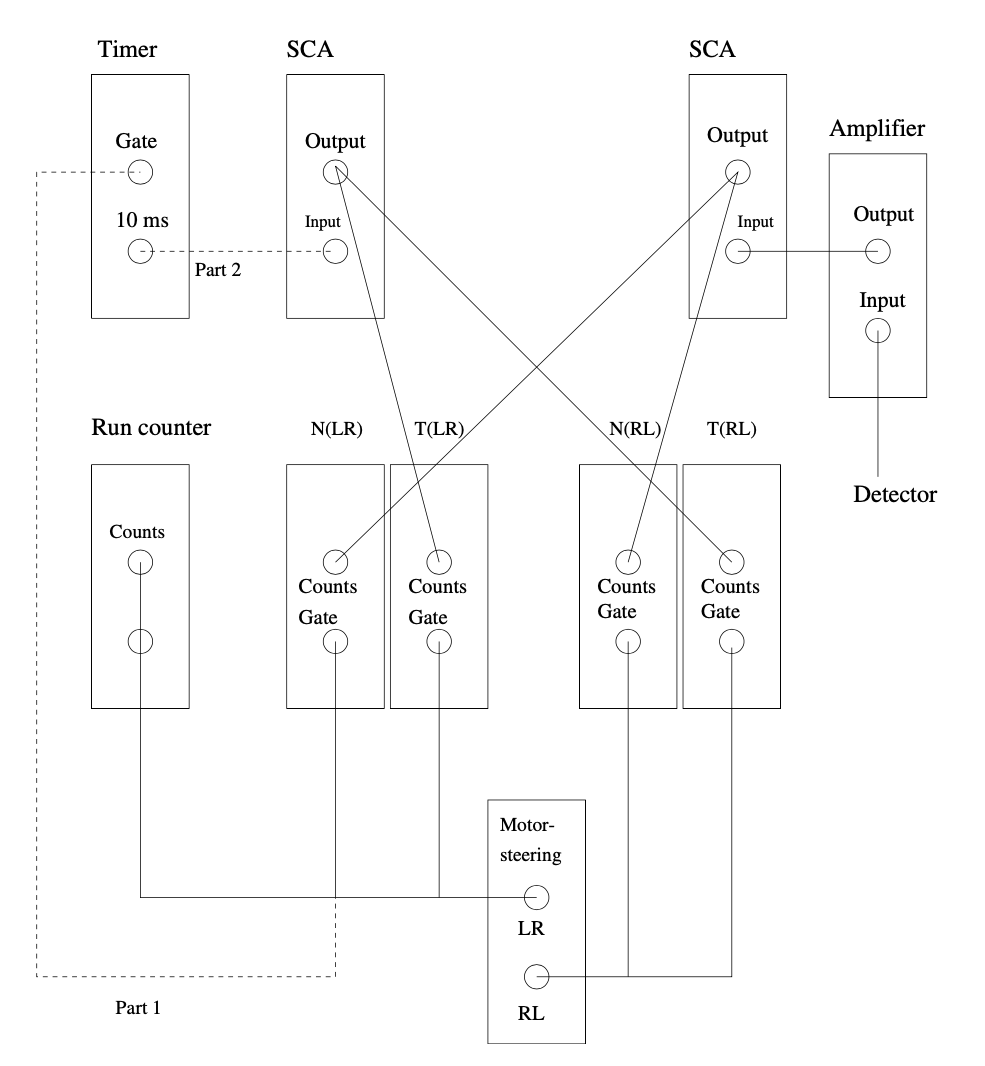
\includegraphics[width=\linewidth]{figs/setup.png}
	\caption{Experimental setup with the two wiring option Part 1 and Part 2 \cite{manual}}\label{fig:setup}
\end{figure}
\newpage
\section{Measurements and Analysis}
In this section we will present our measurement and do the analysis of the data. 
\subsection{Measurement of the $^{57}$Fe $\gamma$-spectrum} 
After the initial setup, we wired the electronics to match Part 1 from scheme \ref{fig:setup}. With this setup we are able to measure the $\gamma$-spectrum of $^{57}$Fe and set a proper window size of the SCA.
To get a sufficient resoluted spectrum, we set the window size to 50 Channel-Units and increased --after every 10s measurement of the counting rate-- the lower limit. Because we couldn't set the potentiometer to 0 Ch. on the SCA, we started at 100 Ch.. We scanned for three lines. The first would be the energy of the electron cascade that happens after the electron capture in the $^{57}$Co at about 6keV, the second should be the \textsc{Mösbauer}-line --that we are searching for-- of 14.4keV and a third small one, that is a result of the simultaneous measuring (detector limitation/coincidences) of the first two lines at the sum of both energies. The resulting histogram is shown in figure \ref{fig:SCA}.

\begin{figure}[H]
	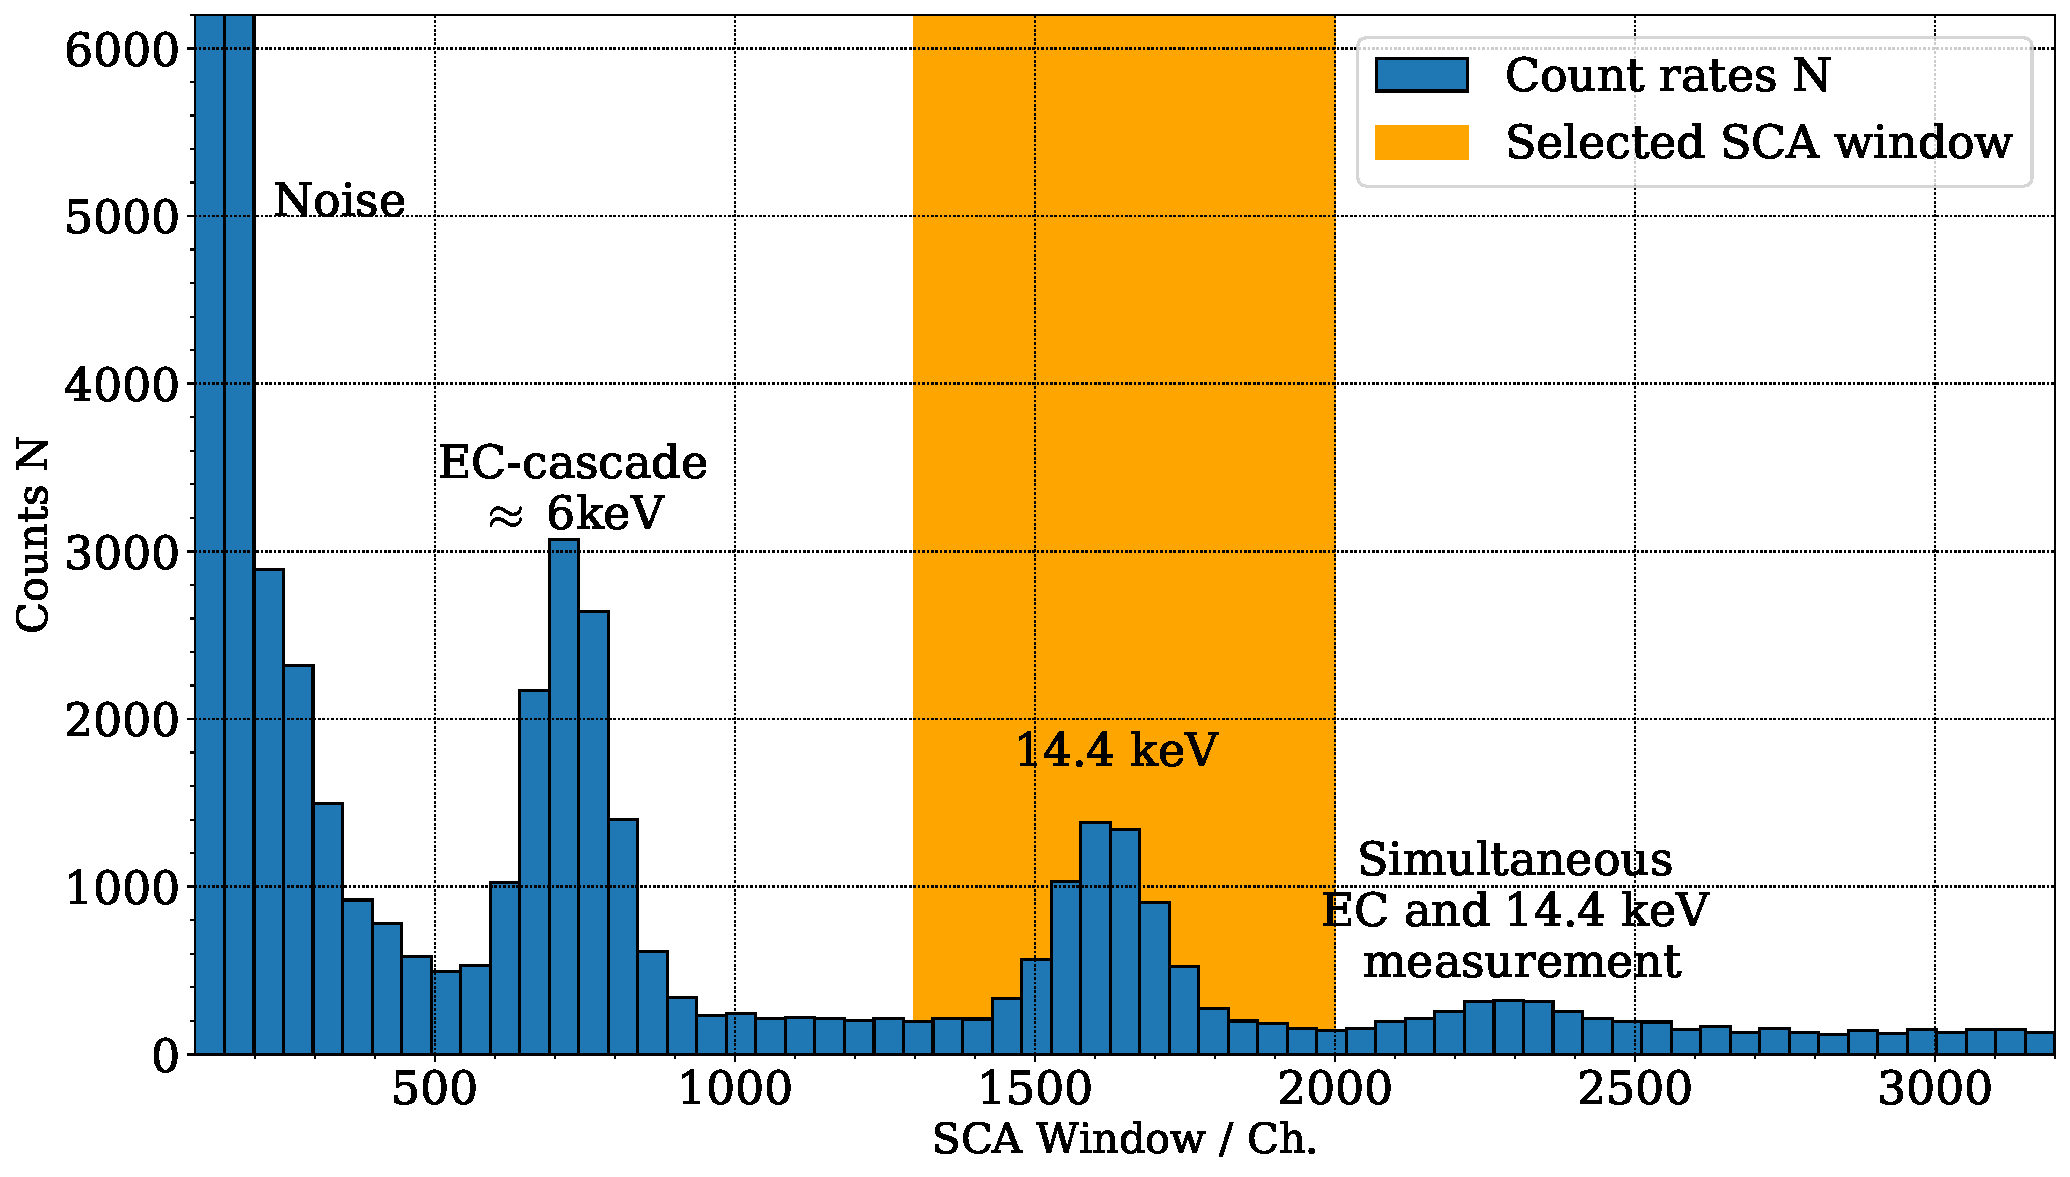
\includegraphics[width=\linewidth]{figs/SCA.pdf}
	\caption{$\gamma$-spectrum of $^{57}$Fe}\label{fig:SCA}
\end{figure}

For the following measurement we set the SCA window to 1300-2000 Ch..

\subsection{Measurement of the \textsc{Mö\ss bauer}-spectrum}\label{sec:doublelinewidth}
After setting the SCA-window, we proceeded by wiring up Part 2 of scheme \ref{fig:setup}. Therefore we applied the gate signal of the timer to the counter NL.

The motorspeed can be set by a potentiometer. We started with the highest possible velocity (2.60 Ch.). One could also start with the slowest but since we didn't know in which velocity space the absorption dips are visible and the velocity is given in units of mm/s, the waiting times for one round would be extremely long. For the coarse measurement of the background we chose 0.04 Ch. steps and for measurements inside the dip 0.02 Ch.. Our goal was to measure for each velocity at least 4000 events s.t. the resulting relative error of the counting rate is $<2\%$. The resulting \textsc{Mösbauer}-spectrum is depicted in figure \ref{fig:moesbauer}.

\begin{figure}[H]
	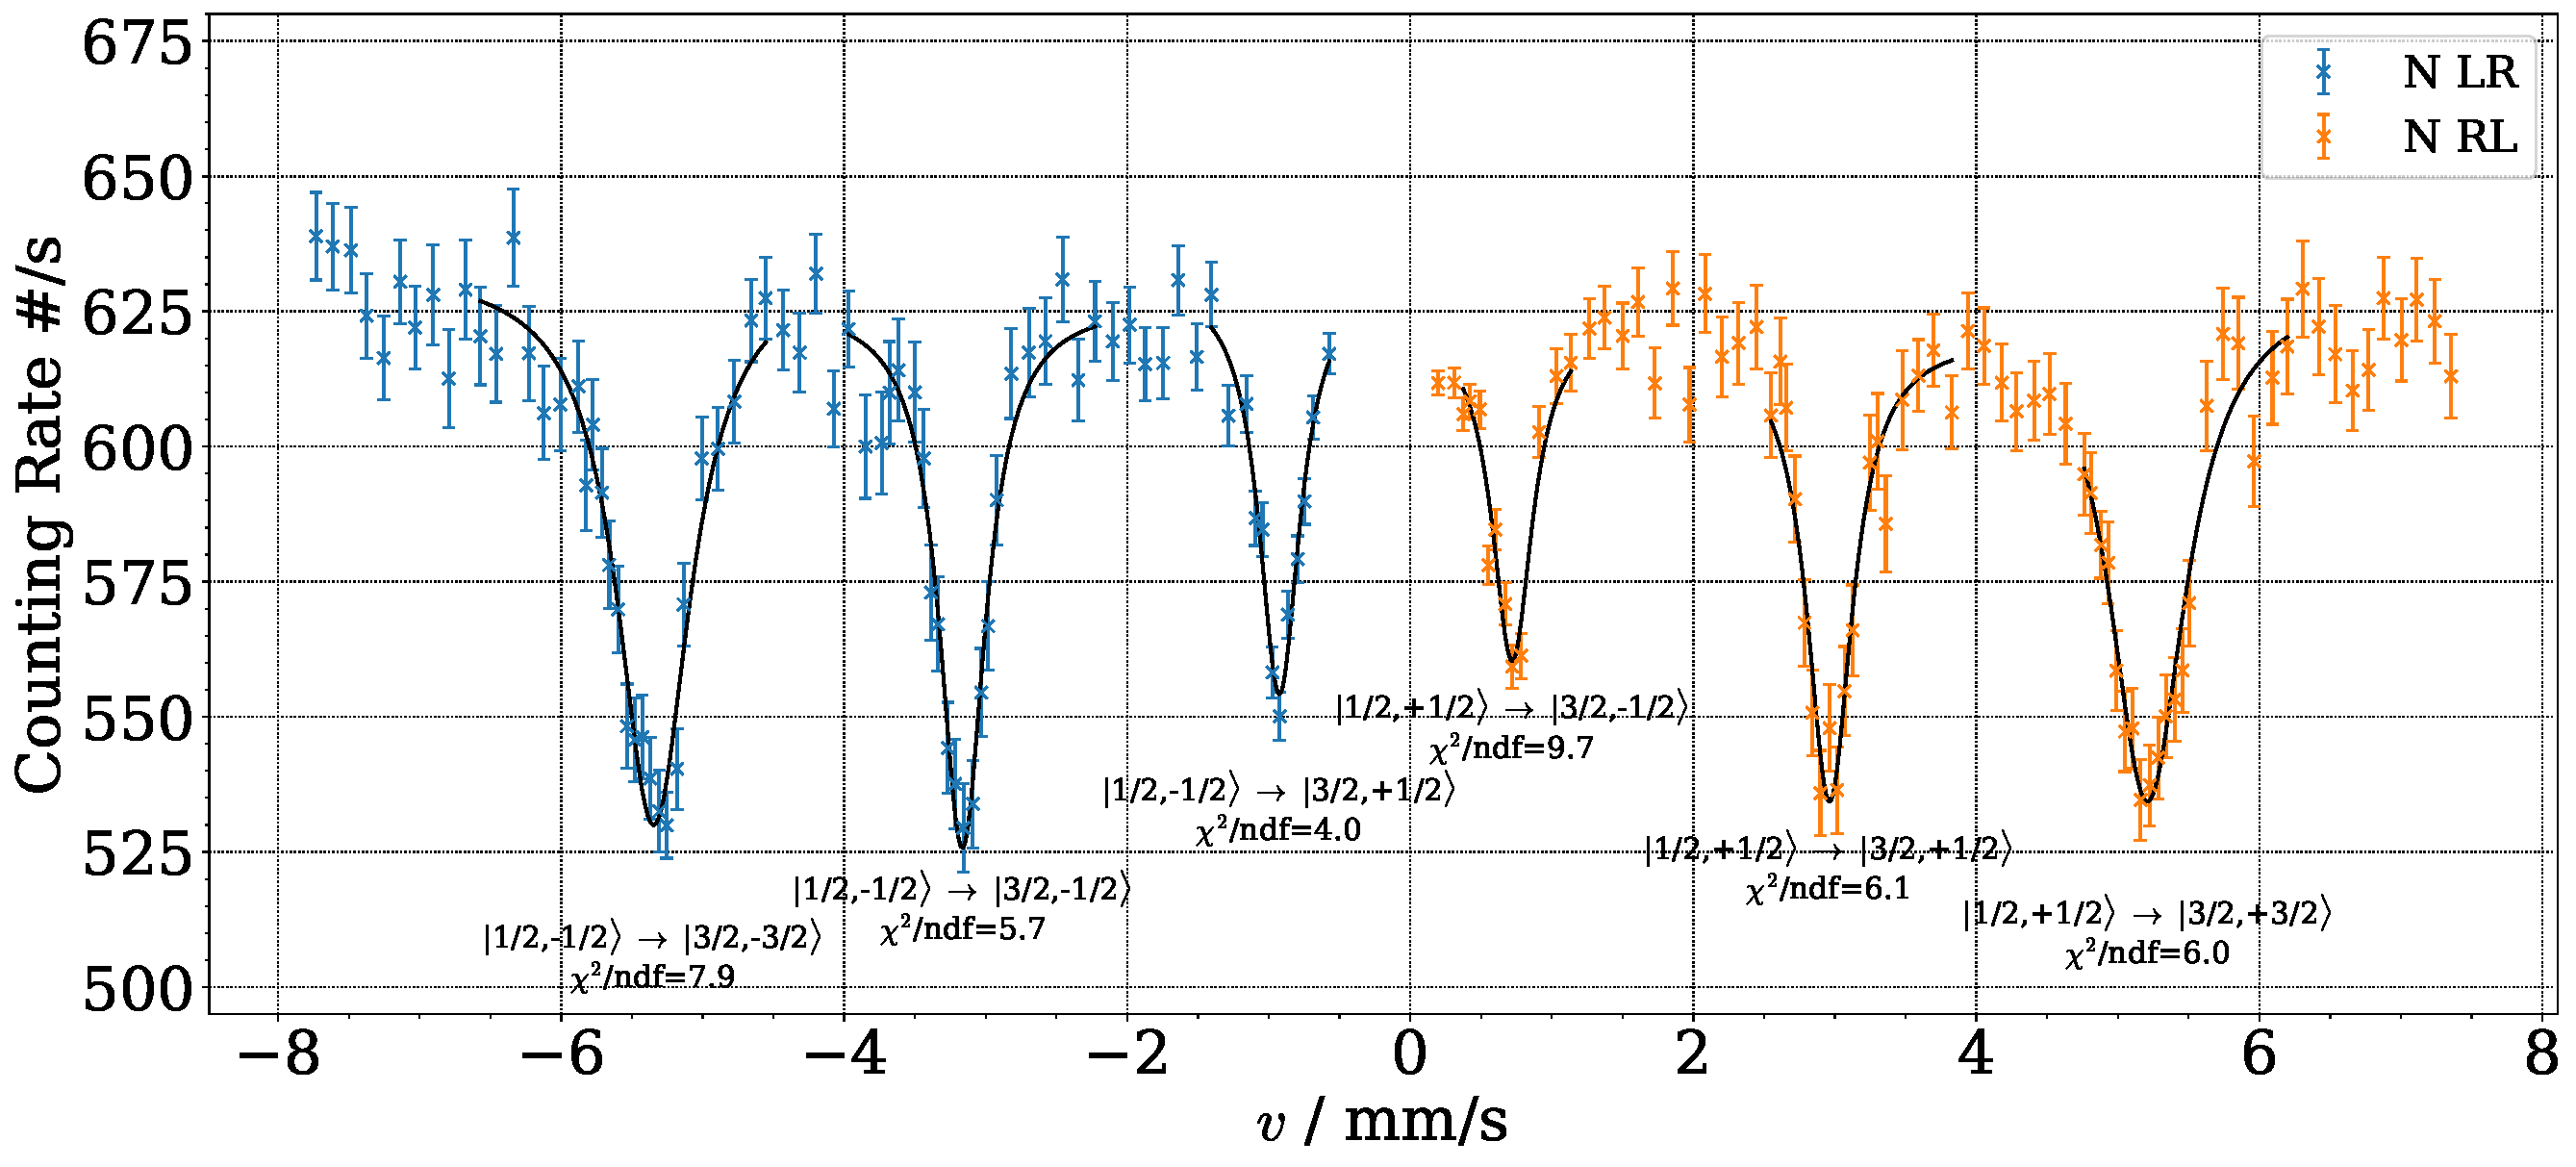
\includegraphics[width=\linewidth]{figs/moesbauer.pdf}
	\caption{ \textsc{Mö\ss bauer}-spectrum of the 14.4keV line of $^{57}$Fe. The dip labels refer to $|I,m_I \rangle$}\label{fig:moesbauer}
\end{figure}

We applied the convention that positive velocities mean approaching source and absorber or in other words, the movements from right to left (RL) \cite{chemistry}. The velocity was calculated from the known distance $s=25.1$mm, the time $t$ and the number of rounds $N_r$. The electronics are set up in away, that a round starts on the left side and makes at least one full round trip. 

One can see that we didn't measure even smaller velocities because of time reasons and the knowledge that there should only be 6 dips for this spectrum. We then fitted the \textsc{Lorentz}-function \cite{demtröder}
\begin{align*}
	f(v)=a\cdot\frac{(\frac{\Gamma}{2})^2}{(v-v_0)^2+(\frac{\Gamma}{2})^2}+b \\
\end{align*}
\begin{center}
	\vspace{-0.8cm}
	$	\text{with the linewidth } \Gamma\text{, the amplitude } a\text{, offset } b\text{ and mean velocity } v_0$
\end{center}
to every dip and ordered them to the associated transitions. The observed linewidth $\Gamma$ is twice as wide as the natural line width \cite{chemistry} \color{red}why?\color{black}. This can be done by assigning the expected relative dip heights --given by the the square of the corresponding $3j$ symbol \cite{chemistry}-- to the measured ones. The derivation of the relation between the relative peak intensity $I$ and the $3j$-symbol $$I(I_e,m_e,I_g,m_g,\sigma lm)\propto\begin{pmatrix}I_g&l&I_e\\-m_g&m&m_e
\end{pmatrix}^2F_{lm}(\theta)$$ would break the boundaries of this report. One can consult for further information the text book \cite{chemistry}. Table \ref{tab:dips} lists all found parameters for every dip and the corresponding $3j$ symbol taken from \cite{chemistry}.

\begin{table}
	\centering
	\begin{tabular}{c|c|c|c|c|c}
	
		Transition $|I,m_I \rangle$ &$3j$-square& $a$&$b$ &$\Gamma$ / mm/s&$v_0$ / mm/s \\
		\hline
		$|1/2,-1/2\rangle \to |3/2,-3/2\rangle$&${3/12}$& -103.3 $\pm$ 5.4 & 633.3 $\pm$ 5.1 & 0.626 $\pm$ 0.071 & -5.346 $\pm$ 0.013\\
		$|1/2,-1/2\rangle\rightarrow |3/2,-1/2\rangle$&${2/12}$& -100.8 $\pm$ 5.6 & 626.5 $\pm$ 3.7 & 0.394 $\pm$ 0.045 & -3.165 $\pm$ 0.010\\
		$|1/2,-1/2\rangle\rightarrow |3/2,+1/2\rangle$&${1/12}$& -76.8 $\pm$ 6.6 & 630.9 $\pm$ 6.8 & 0.350 $\pm$ 0.055 & -0.925 $\pm$ 0.009\\
		$|1/2,+1/2\rangle\rightarrow |3/2,+3/2\rangle$&${3/12}$& -95.5 $\pm$ 7.3 & 629.9 $\pm$ 7.5 & 0.662 $\pm$ 0.090 & 5.209 $\pm$ 0.014\\
		$|1/2,+1/2\rangle\rightarrow |3/2,+1/2\rangle$&${2/12}$& -85.8 $\pm$ 6.7 & 620.0 $\pm$ 5.3 & 0.387 $\pm$ 0.065 & 2.963 $\pm$ 0.014\\
		$|1/2,+1/2\rangle\rightarrow |3/2,-1/2\rangle$&${1/12}$ & -63.1 $\pm$ 10.3& 623.4 $\pm$ 10.9 & 0.348 $\pm$ 0.116 & 0.720 $\pm$ 0.020\\
		\hline
	\end{tabular}
	\caption{Fit parameters for the associated dips}\label{tab:dips}
\end{table}

Differences in velocity can be transferred in units of energy by \cite{chemistry}:
$$dE=\frac{dE}{dv} dv=\frac{E}{c}dv\Rightarrow \Delta E=\frac{14.4keV}{c}\Delta v$$

\subsection{Line widths}
After the conversion into units of energy the  parameters of interest from table \ref{tab:dips} become
\begin{table}[H]
	\centering
	\begin{tabular}{c|c|c}
		Transition $|I,m_I \rangle$ &$\Gamma$ / neV &$E_0$ / neV \\
		\hline
			|1/2,-1/2$\rangle$ $\rightarrow$ |3/2,-3/2$\rangle$& 30.068 $\pm$ 3.414 & -256.623 $\pm$ 0.633\\
			|1/2,-1/2$\rangle$ $\rightarrow$ |3/2,-1/2$\rangle$& 18.907 $\pm$ 2.147 & -151.934 $\pm$ 0.481\\
			|1/2,-1/2$\rangle$ $\rightarrow$ |3/2,+1/2$\rangle$& 16.814 $\pm$ 2.630 & -44.405 $\pm$ 0.427\\
			|1/2,+1/2$\rangle$ $\rightarrow$ |3/2,+3/2$\rangle$& 31.793 $\pm$ 4.331 & 250.018 $\pm$ 0.677\\
			|1/2,+1/2$\rangle$ $\rightarrow$ |3/2,+1/2$\rangle$ & 18.582 $\pm$ 3.140 & 142.210 $\pm$ 0.657\\
			|1/2,+1/2$\rangle$ $\rightarrow$ |3/2,-1/2$\rangle$& 16.720 $\pm$ 5.555 & 34.562 $\pm$ 0.937\\
		\hline
	\end{tabular}
	\caption{Fit parameters for the associated dips}\label{tab:dips_energy}
\end{table}
and the spectrum looks as depicted in figure  \ref{fig:mosbauer_energy}.
\begin{figure}[H]
	\centering
	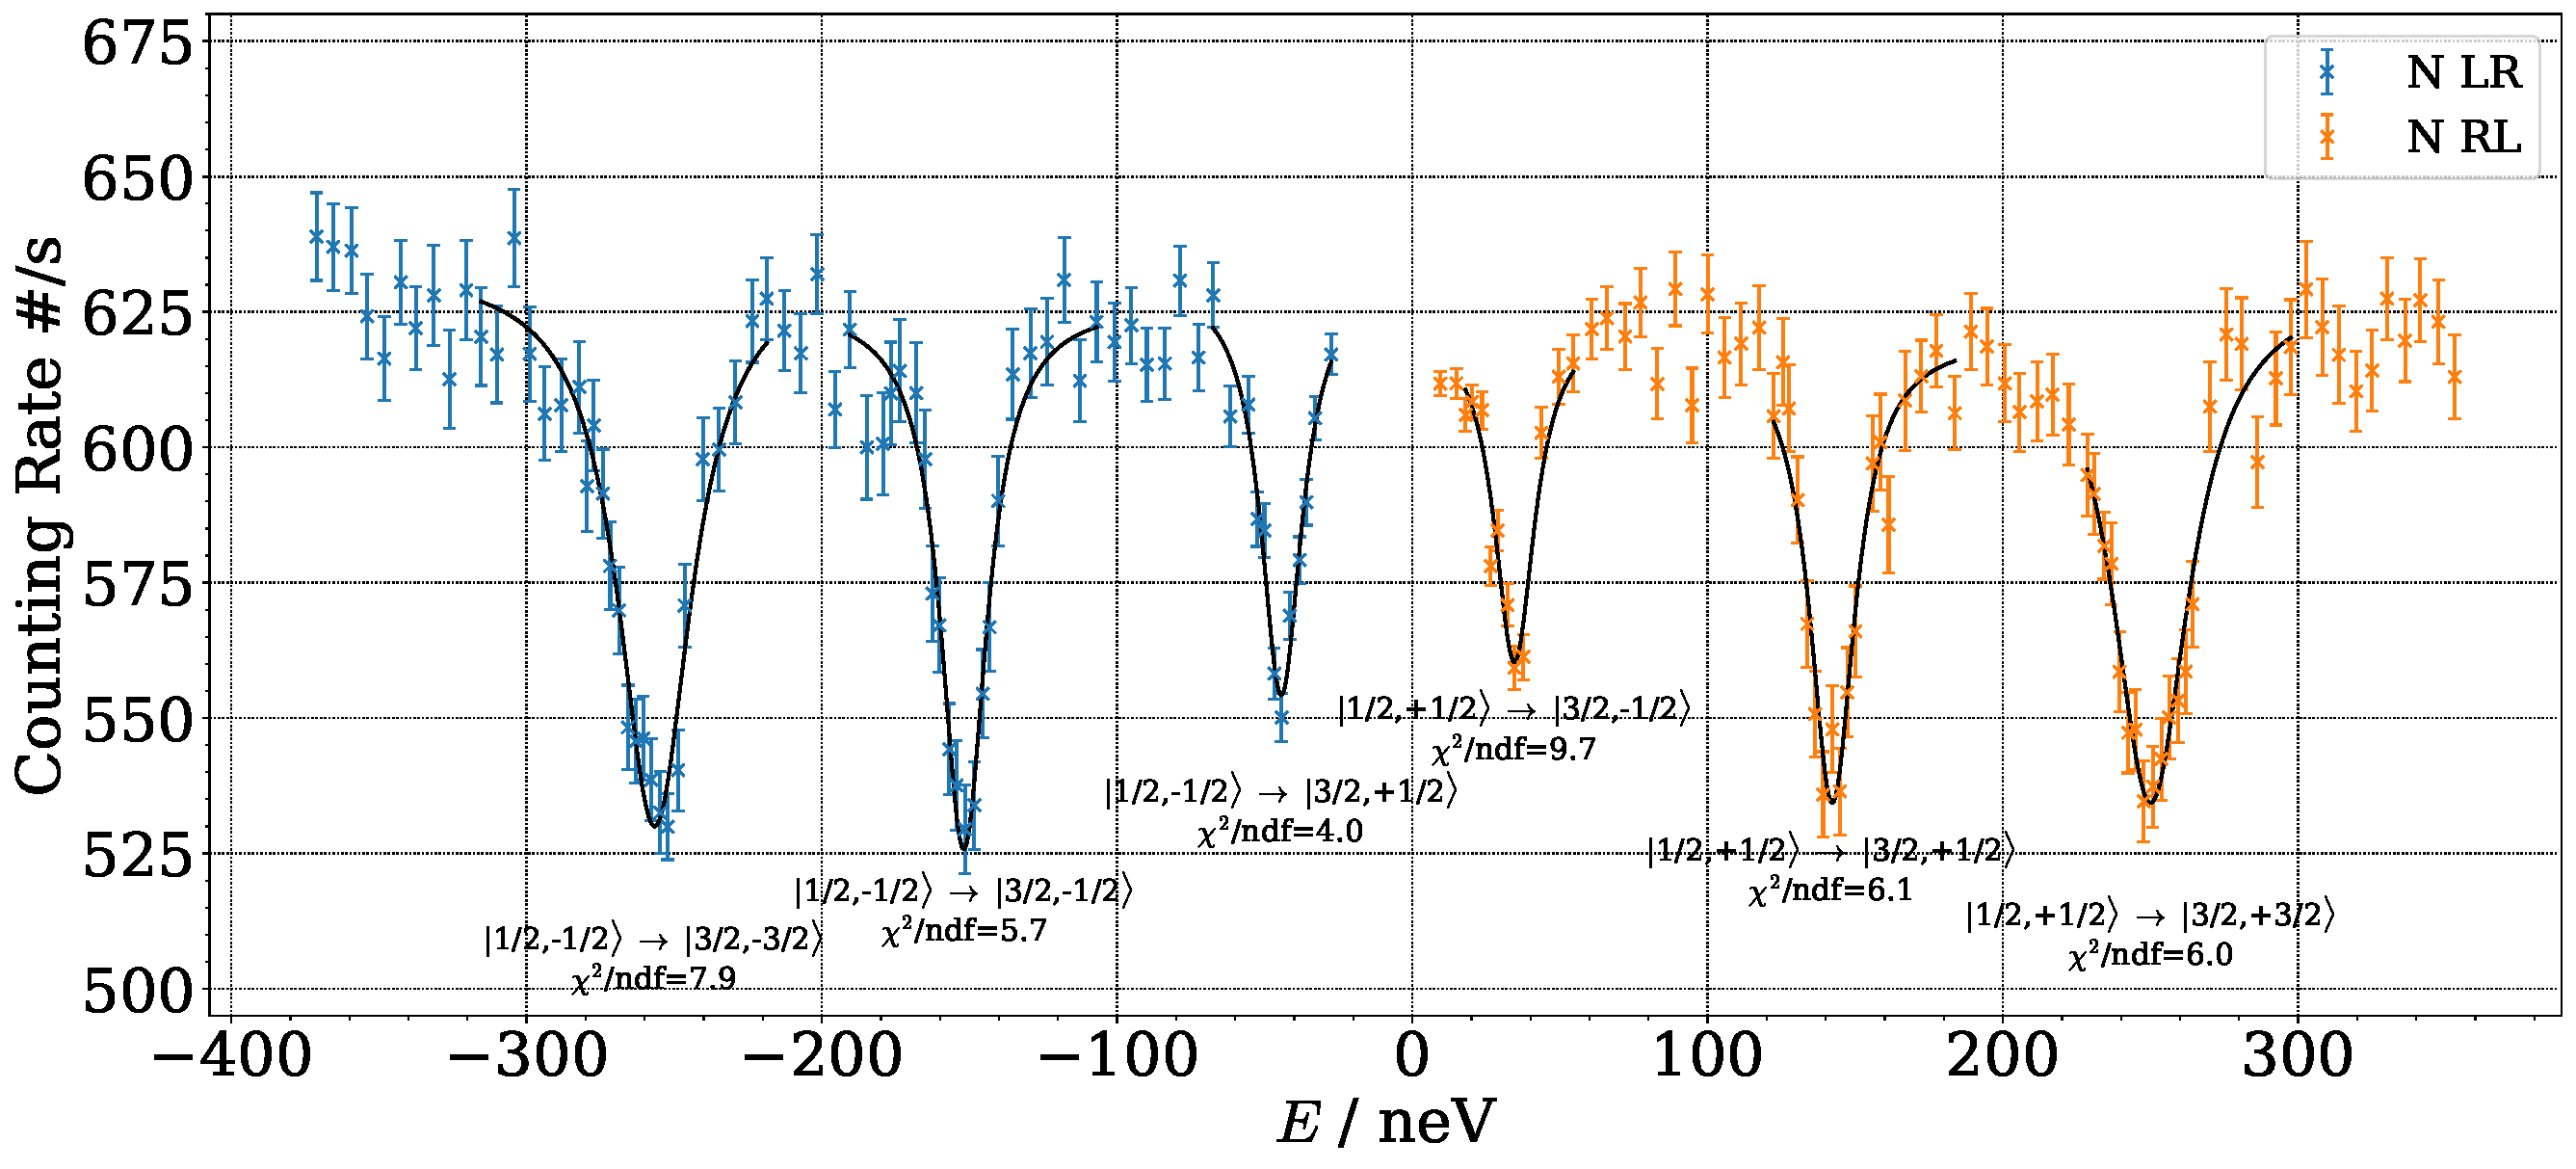
\includegraphics[width=\linewidth]{figs/moesbauer_energy.pdf}
	\caption{\textsc{Mö\ss bauer}-spectrum of the 14.4keV line of $^{57}$Fe in units of energy. The dip labels refer to $|I,m_I \rangle$}\label{fig:mosbauer_energy}
\end{figure}
The observed double linewidths lie between around  17 neV and 31 neV. As motivated in section \ref{sec:doublelinewidth} the linewidth of the absorption/emission only is the half measured width and lies between 8.5 neV and 15.5 neV. The known natural linewidth of the $^{57}$Fe is 4.7neV \cite{schatz} and therefore only 1.8-3.3 times smaller than our measurement. The broadening can be the result of a \textsc{Debye-Waller}-factor $f$ that is <1. The tutor suggested that the factor is less then $80\%$ --our estimation from section \ref{sec:debye} was $f\approx0.78$-- which means that round 20\% of all photons --emitted and absorbed-- loose energy on phonons on either the source or the target material. The material choice, even with this \textsc{Debye-Waller}-factor is sufficient, since it doesn't require cooling and has long livetimes. A material with $f=1$ can't be found even at temperatures of $T=0$K due to zero-point energy. \cite{schatz}
\subsection{The $g$-factor}
Now we want to derive the $g$-factors for the excited and ground state $g_{3/2}$ and  $g_{1/2}$ from our data. 

For the magnetic field of the $^{57}$Fe we assume $H=(333 \pm10)\text{kG}=(33.3\pm 1.0)$T \cite{manual} and use the literature value for the nuclear magneton $\mu_N=3.152451\cdot 10^{-8}$eVT$^{-1}$ \cite{magneton} to derive with equation \eqref{eq:hyperfine} the relations
\begin{align*}
	g_{1/2}=-\frac{\Delta E_{1/2}}{\mu_N\cdot B} && g_{3/2}=-\frac{\Delta E_{3/2}}{\mu_N\cdot B}
\end{align*}
for splittings with $\Delta m_I=1$ and the associated energy difference $\Delta E_I$. 

Our choice for the transitions depends --as explained in \ref{sec:spectrum}-- on the fact, that we want to cancel out the quadrupole shift. Since for the ground state a quadrupole shift doesn't exist, we chose the transitions to the excited states $m_{3/2}=\pm 1/2$. The choice of states is intuitively depicted in figure \ref{fig:hyperfine}. We find for each $g$-factor  two energy differences $\Delta E_I$:
\begin{align*}
	\Delta E_{1/2}=\begin{cases}
		E(|1/2,+1/2\rangle\to|3/2,-1/2\rangle)-E(|1/2,-1/2\rangle\to|3/2,-1/2\rangle)\\
		E(|1/2,+1/2\rangle\to|3/2,+1/2\rangle)-E(|1/2,-1/2\rangle\to|3/2,+1/2\rangle)\\		
	\end{cases}	\\
	\Delta E_{3/2}=\begin{cases}
		E(|1/2,-1/2\rangle\to|3/2,+1/2\rangle)-E(|1/2,-1/2\rangle\to|3/2,-1/2\rangle)\\
		E(|1/2,+1/2\rangle\to|3/2,+1/2\rangle)-E(|1/2,+1/2\rangle\to|3/2,-1/2\rangle)\\		
	\end{cases}	
\end{align*}
By averaging those energies, one finds:
\begin{align*}
	\Delta E_{1/2}=(-186.56 \pm 0.66)\text{neV} &\Rightarrow g_{1/2}=0.1777 \pm 0.0049\\ \Delta E_{3/2}=(107.59 \pm 0.66)\text{neV}&\Rightarrow g_{3/2}=-0.1025 \pm 0.0038
\end{align*}
To set the found values in comparison to the literature \cite{gfactor}, we take the ratio between both found factors $g_I$:

\begin{align*}
	G_{\text{exp.}}=\frac{g_{1/2}}{g_{3/2}}=-1.734 \pm 0.0625 &&G_{\text{lit.}}=-1.715\pm0.004
\end{align*}
The literature value of $G_{lit.}$ lies within the error of our result. Besides this deviates our result by just $\approx1\%$ from the literature value. This is a surprising accurate result.
\newpage
\subsection{Isomeric shift}
By inverting the sign of the energies for LR, one can see that the spectrum isn't perfectly symmetric (see \ref{fig:asymm}). This results from the isomeric shift that shifts the whole spectrum by $\Delta E_{\text{iso}}$.


One can then derive the isometric shift by calculating the shifts between each peak and his presumptive mirrored one. Since the signs of LR and RL are opposite this is the same as the average of all peak positions. With this in mind we find the isomeric shift
$$\Delta E_{\text{iso.}}=(-4.36\pm0.80)\text{neV}$$
The isomeric shift is probably the result of the different materials that the $^{57}$Co respectively $^{57}$Fe probes are held in. 

\begin{figure}[H]%[14]{R}{0.45\textwidth}
	%\vspace{-1cm}
	\centering
	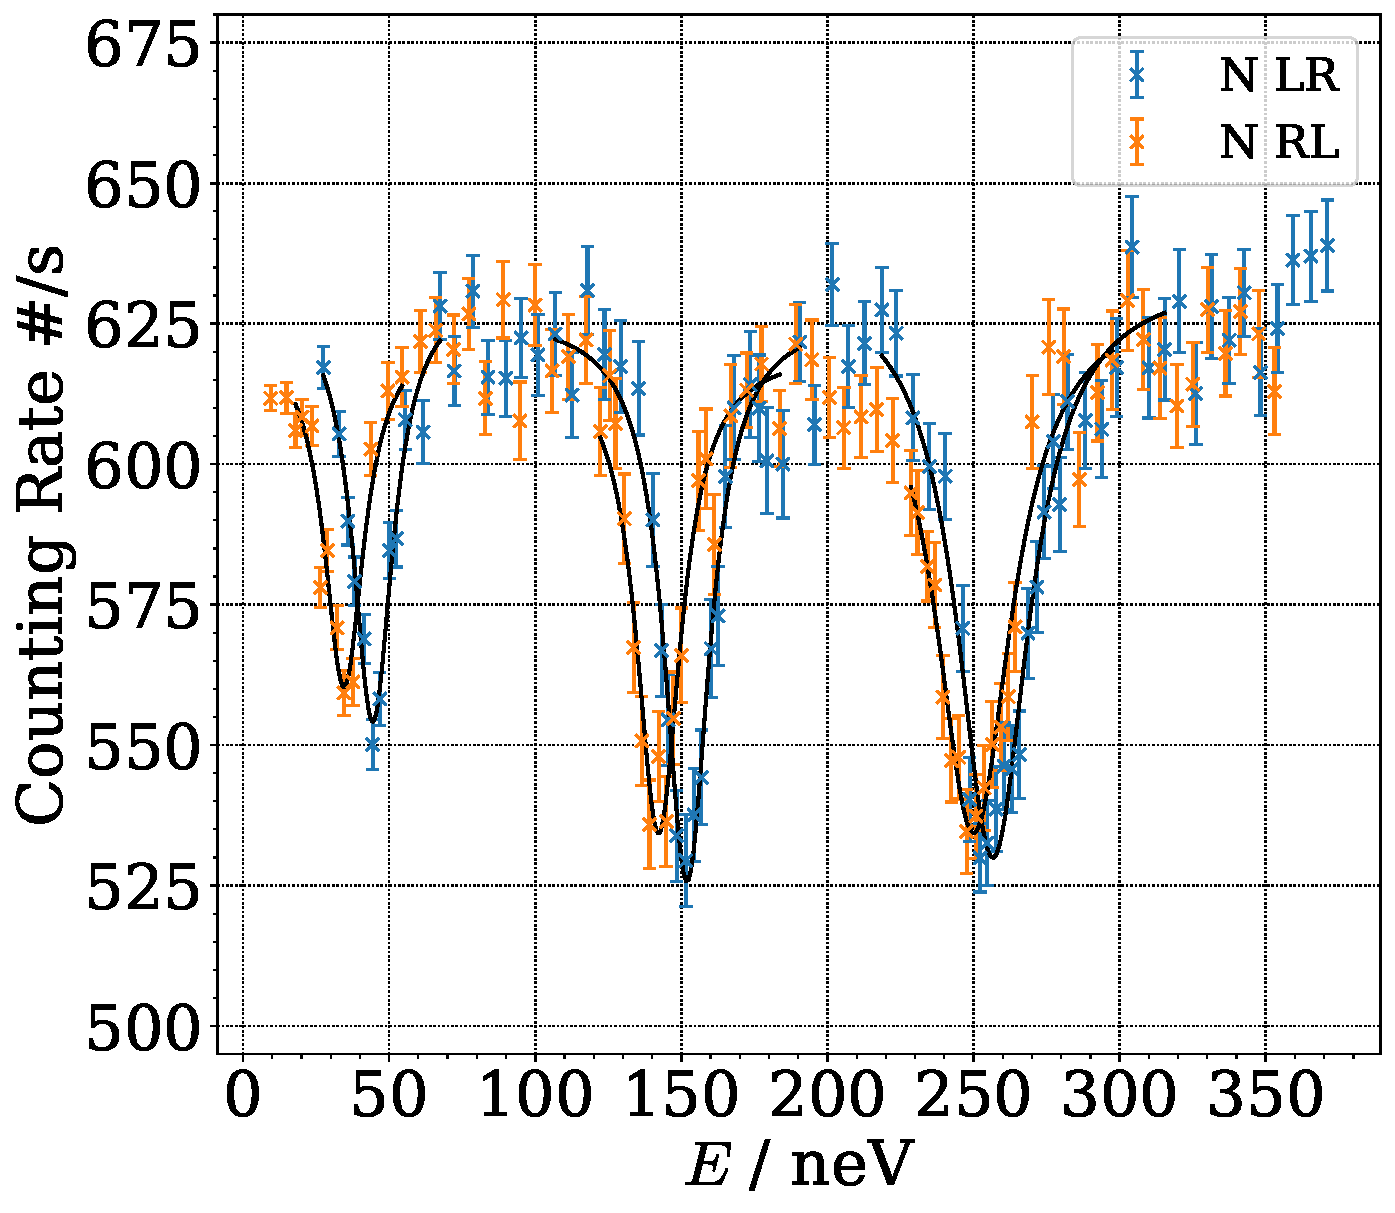
\includegraphics[width=0.7\linewidth]{figs/moesbauer_mirrored.pdf}
	\caption{Mirrored LR measurement to visualize isomeric shift}\label{fig:asymm}
\end{figure}
\newpage
\section{Conclusion}
In this lab course we investigated the recoilless absorption/emission called \textsc{Mö\ss bauer}-effect. We started with taking a coarse $\gamma$-spectrum to find the 14.4keV transition of $^{57}$Fe to calibrate the window of a single channel analyzer. Afterwards we measured with a source and a moving absorber the so called \textsc{Mö\ss bauer}-spectrum that includes visible effects of electric and magnetic multipole effects.

One derived property of this spectrum is the natural linewidth, which was determined for the hyperfine structure and lied between 8.5neV and 15.5neV. Therefor was our result about 1.8-3.3 times larger then the known linewidth of 4.7neV \cite{schatz}.

From the resulting \textsc{Mö\ss bauer}-spectrum we obtained the $g$-factor for the ground state and excited state as:
\begin{align*}
	g_{1/2}=0.1777 \pm 0.0049 &&g_{3/2}=-0.1025 \pm 0.0038
\end{align*}
and compared the ratio of them to the literature value from \cite{gfactor}:
\begin{align*}
	G_{\text{exp.}}=\frac{g_{1/2}}{g_{3/2}}=-1.734 \pm 0.0625 &&G_{\text{lit.}}=-1.715\pm0.004
\end{align*}
Last but not least we investigated the isomeric shift that shifts the whole spectrum by the energy
$$\Delta E_{\text{iso.}}=(4.36\pm0.80)\text{neV}$$

The overall results are impressive, especially if one takes the small dimensions of the experiment and the slow velocities into account. We could have decreased the errors by measuring longer since the error of counts $N$ goes with $\sqrt{N}$. The experiment was long not in use, therefore the electronics could have suffered from thermal influences. We countered this by letting it run for a few minutes before taking any measurements. The influence of thermal fluctuation was not significant.
\newpage
\section{Appendix}

\subsection{Remark on measurement errors}
We measured counts throughout the whole experiment. Every count $N$ is associated with an error $\sigma_N=\sqrt{N}$ (\textsc{Poisson} statistics). All errors are propagated using \textsc{Gaussian} error propagation.


\subsection{Measured data}
All data we measured was visualized in this report only in the form of plots. If there is need to view the data in detail it can be found in our \href{https://github.com/krausejm/advanced_lab_course}{GitHub repository}. 

\begin{table}[H]
	\centering
	\begin{tabular}{c|c|c|c}
		lower limit / Ch. & upper limit / Ch. & {counts} $N$ & {time} $t$ / s \\
		\hline
		{100}               & 50                         & 71770           & 10           \\
		{150}               & 200                        & 6954            & 10           \\
		{200}               & 250                        & 2893            & 10           \\
		{250}               & 300                        & 2317            & 10           \\
		{300}               & 350                        & 1499            & 10           \\
		{350}               & 400                        & 921             & 10           \\
		{400}               & 450                        & 780             & 10           \\
		{450}               & 500                        & 585             & 10           \\
		{500}               & 550                        & 495             & 10           \\
		{550}               & 600                        & 529             & 10           \\
		{600}               & 650                        & 1024            & 10           \\
		{650}               & 700                        & 2170            & 10           \\
		{700}               & 750                        & 3072            & 10           \\
		{750}               & 800                        & 2642            & 10           \\
		{800}               & 850                        & 1402            & 10           \\
		{850}               & 900                        & 612             & 10           \\
		{900}               & 950                        & 337             & 10           \\
		{950}               & 1000                       & 230             & 10           \\
		{1000}              & 1050                       & 246             & 10           \\
		{1050}              & 1100                       & 212             & 10           \\
		{1100}              & 1150                       & 221             & 10           \\
		{1150}              & 1200                       & 212             & 10           \\
		{1200}              & 1250                       & 201             & 10           \\
		{1250}              & 1300                       & 215             & 10           \\
		{1300}              & 1350                       & 197             & 10           \\
		{1350}              & 1400                       & 213             & 10           \\
		{1400}              & 1450                       & 211             & 10           \\
		{1450}              & 1500                       & 331             & 10           \\
		{1500}              & 1550                       & 568             & 10           \\
		{1550}              & 1600                       & 1029            & 10           \\
		{1600}              & 1650                       & 1382            & 10           \\
		{1650}              & 1700                       & 1340            & 10           \\
		{1700}              & 1750                       & 905             & 10           \\
		{1750}              & 1800                       & 525             & 10           \\
		{1800}              & 1850                       & 275             & 10           \\
		{1850}              & 1900                       & 199             & 10           \\
		{1900}              & 1950                       & 185             & 10           \\
		{1950}              & 2000                       & 156             & 10           \\
		{2000}              & 2050                       & 145             & 10           \\
		{2050}              & 2100                       & 157             & 10           \\
		{2100}              & 2150                       & 197             & 10           \\
		{2150}              & 2200                       & 216             & 10           \\
		{2200}              & 2250                       & 258             & 10           \\
		{2250}              & 2300                       & 314             & 10           \\
	\end{tabular}
	\caption{Data of Part 1}
\end{table}
\begin{table}[H]
	\ContinuedFloat
	\centering
	\begin{tabular}{c|c|c|c}
		lower limit / Ch. & upper limit / Ch. & {counts} $N$ & {time} $t$ / s\\
		\hline
		{2300}              & 2350                       & 323             & 10           \\
		{2350}              & 2400                       & 314             & 10           \\
		{2400}              & 2450                       & 258             & 10           \\
		{2450}              & 2500                       & 214             & 10           \\
		{2500}              & 2550                       & 197             & 10           \\
		{2550}              & 2600                       & 193             & 10           \\
		{2600}              & 2650                       & 151             & 10           \\
		{2650}              & 2700                       & 169             & 10           \\
		{2700}              & 2750                       & 131             & 10           \\
		{2750}              & 2800                       & 152             & 10           \\
		{2800}              & 2850                       & 128             & 10           \\
		{2850}              & 2900                       & 120             & 10           \\
		{2900}              & 2950                       & 142             & 10           \\
		{2950}              & 3000                       & 126             & 10           \\
		{3000}              & 3050                       & 151             & 10           \\
		{3050}              & 3100                       & 129             & 10           \\
		{3100}              & 3150                       & 146             & 10           \\
		{3150}              & 3200                       & 146             & 10           \\
		{3200}              & 3250                       & 131             & 10          
	\end{tabular}
	\caption{Data of Part 1}
\end{table}

\begin{table}[H]
	\centering
	\begin{tabular}{c|c|c|c|c|c}
		Velocity / Ch. & rounds & $t_{LR}$  / 10ms & $N_{LR}$  &$t_{RL}$  / 10m & $N_{RL}$  \\
		\hline
		2.6  & 3      & 974         & 6223  & 1024        & 6277  \\
		2.56 & 3      & 989         & 6300  & 1040        & 6481  \\
		2.52 & 3      & 1006        & 6401  & 1059        & 6642  \\
		2.48 & 3      & 1021        & 6373  & 1075        & 6662  \\
		2.44 & 3      & 1038        & 6398  & 1095        & 6871  \\
		2.4  & 3      & 1055        & 6652  & 1112        & 6830  \\
		2.36 & 3      & 1071        & 6662  & 1131        & 6903  \\
		2.32 & 2      & 727         & 4566  & 768         & 4739  \\
		2.28 & 2      & 739         & 4527  & 782         & 4865  \\
		2.24 & 2      & 752         & 4730  & 796         & 5008  \\
		2.2  & 2      & 764         & 4740  & 810         & 5010  \\
		2.16 & 2      & 777         & 4795  & 824         & 5049  \\
		2.12 & 2      & 792         & 5058  & 842         & 5029  \\
		2.08 & 2      & 806         & 4975  & 858         & 5312  \\
		2.04 & 2      & 820         & 4971  & 874         & 5426  \\
		2    & 2      & 836         & 5081  & 892         & 5419  \\
		1.96 & 2      & 854         & 5219  & 912         & 5208  \\
		1.94 & 2      & 862         & 5110  & 920         & 5139  \\
		1.92 & 2      & 869         & 5249  & 929         & 5139  \\
	\end{tabular}
	\caption{Data of Part 2}
\end{table}


\begin{table}[H]
	\centering
	\ContinuedFloat
	\begin{tabular}{c|c|c|c|c|c}
		Velocity / Ch. & rounds & $t_{LR}$  / 10ms & $N_{LR}$  &$t_{RL}$  / 10m & $N_{RL}$  \\
		\hline
		1.90 & 2      & 879         & 5199  & 940         & 5171  \\
		1.88 & 2      & 887         & 5128  & 950         & 5153  \\
		1.86 & 2      & 897         & 5112  & 961         & 5164  \\
		1.84 & 2      & 907         & 4973  & 973         & 5202  \\
		1.82 & 2      & 916         & 4999  & 984         & 5391  \\
		1.8  & 2      & 925         & 5053  & 994         & 5440  \\
		1.78 & 2      & 935         & 5036  & 1006        & 5619  \\
		1.76 & 2      & 946         & 5038  & 1018        & 5889  \\
		1.74 & 3      & 1433        & 7594  & 1543        & 8977  \\
		1.72 & 2      & 969         & 5236  & 1044        & 6174  \\
		1.70 & 2      & 978         & 5582  & 1054        & 6270  \\
		1.66 & 2      & 1003        & 5996  & 1084        & 6549  \\
		1.62 & 2      & 1026        & 6152  & 1111        & 6774  \\
		1.58 & 2      & 1051        & 6393  & 1139        & 6930  \\
		1.54 & 2      & 1078        & 6719  & 1172        & 7108  \\
		1.50 & 2      & 1102        & 6915  & 1201        & 7348  \\
		1.46 & 2      & 1133        & 7042  & 1238        & 7658  \\
		1.42 & 2      & 1163        & 7180  & 1274        & 7916  \\
		1.38 & 2      & 1195        & 7552  & 1312        & 7955  \\
		1.34 & 2      & 1232        & 7478  & 1358        & 8390  \\
		1.30 & 2      & 1265        & 7865  & 1398        & 8572  \\
		1.26 & 1      & 652         & 3912  & 722         & 4394  \\
		1.22 & 1      & 672         & 4036  & 747         & 4375  \\
		1.2  & 1      & 682         & 4160  & 760         & 4567  \\
		1.18 & 1      & 694         & 4262  & 773         & 4615  \\
		1.14 & 1      & 717         & 4374  & 803         & 4545  \\
		1.12 & 1      & 730         & 4364  & 818         & 4538  \\
		1.1  & 1      & 741         & 4246  & 832         & 4463  \\
		1.08 & 1      & 752         & 4265  & 847         & 4641  \\
		1.06 & 1      & 768         & 4180  & 866         & 4641  \\
		1.04 & 1      & 780         & 4193  & 883         & 4863  \\
		1.02 & 1      & 795         & 4209  & 901         & 5112  \\
		1.0  & 1      & 812         & 4335  & 923         & 5448  \\
		0.98 & 1      & 828         & 4591  & 945         & 5738  \\
		0.96 & 1      & 841         & 4767  & 960         & 5911  \\
		0.94 & 1      & 859         & 5069  & 985         & 5967  \\
		0.9  & 1      & 890         & 5460  & 1026        & 6383  \\
		0.86 & 1      & 932         & 5754  & 1082        & 6699  \\
		0.82 & 1      & 974         & 6034  & 1139        & 7023  \\
		0.78 & 1      & 1022        & 6448  & 1205        & 7571  \\
		0.74 & 1      & 1070        & 6551  & 1272        & 7730  \\
		0.70 & 1      & 1127        & 7023  & 1353        & 8514  \\
		0.66 & 1      & 1194        & 7396  & 1453        & 8888  \\
		0.62 & 1      & 1266        & 7881  & 1560        & 9777  \\
		0.58 & 1      & 1340        & 8245  & 1672        & 10374 \\
	\end{tabular}
	\caption{Data of Part 2}
\end{table}

\begin{table}[H]
	\centering
	\ContinuedFloat
	\begin{tabular}{c|c|c|c|c|c}
		Velocity / Ch. & rounds & $t_{LR}$  / 10ms & $N_{LR}$  &$t_{RL}$  / 10m & $N_{RL}$  \\
		\hline
		0.54 & 1      & 1437        & 8844  & 1828        & 11404 \\
		0.50 & 1      & 1531        & 9657  & 1984        & 12337 \\
		0.46 & 1      & 1665        & 10266 & 2213        & 13621 \\
		0.42 & 1      & 1786        & 11218 & 2431        & 14903 \\
		0.38 & 1      & 1954        & 11835 & 2757        & 16616 \\
		0.34 & 1      & 2169        & 13185 & 3203        & 17977 \\
		0.32 & 1      & 2295        & 13466 & 3488        & 19508 \\
		0.30 & 1      & 2404        & 14054 & 3742        & 21362 \\
		0.28 & 1      & 2575        & 14374 & 4172        & 24389 \\
		0.26 & 1      & 2715        & 14935 & 4551        & 26305 \\
		0.24 & 1      & 2902        & 16509 & 5102        & 30959 \\
		0.22 & 1      & 3156        & 18279 & 5950        & 36199 \\
		0.20 & 1      & 3354        & 19782 & 6704        & 40624 \\
		0.18 & 1      & 3665        & 22187 & 8092        & 49508 \\
		0.14 & 1      & 4385        & 27063 & 12765       & 78090
	\end{tabular}
	\caption{Data of Part 2}
\end{table}
\newpage

\label{sec:conc}
\printbibliography[heading=bibintoc]
\end{document}
